%% Generated by scripts/build_manuscript.py from docs/paper/MANUSCRIPT.md -- do not edit.
\documentclass[referee,lineno,pdflatex,sn-basic]{sn-jnl}
\usepackage{graphicx,booktabs,tabularx,amsmath,amssymb,xcolor,tikz,url}
\renewcommand{\tabularxcolumn}[1]{>{\raggedright\arraybackslash}p{#1}}
\usetikzlibrary{arrows.meta,positioning,fit}
\raggedbottom
\begin{document}
\title[The Price of Utility]{The Price of Utility: Verification Leverage in Useful-Work Browser Admission}
\author{\fnm{Authors withheld for double-anonymous review}}
\abstract{Proof-of-work challenges protect websites by making visitors spend computation that is then discarded. We measure the price of making that computation useful, on two workload classes, under a protocol whose predictions were committed before each experiment. In the first, each admission carries bounded AutoDock Vina docking units that join a virtual screening campaign and are verified by exactly replaying a secretly sampled unit. Decomposed searches preserved screening accuracy and reproduced bit for bit on phones; with trace commitment and three easily overlooked scheduler fixes, attackers paid about what honest clients pay even with free identities, and rescoring stopped fabricated energies from reordering results. The price is verification: each audit is a molecular replay, so under attack verifier capacity decides who is admitted and budget phones are denied first. Protecting them needed about five replay cores per attacker core, while the same queue with proof-of-work verification served every device class. In the second class, image classifiers for data labelling are verified algebraically in milliseconds and stay available under attack, but verifying them costs the server about as much as computing them, even batched or natively optimised. In both workloads we measured, work worth delegating was expensive to verify and work cheap to verify was not worth delegating.}
\keywords{proof of work, useful work, admission control, CAPTCHA alternatives, verifiable computation, denial of service, result verification, molecular docking, data labelling}
\maketitle

\section{Introduction}

Websites that cannot tell people from programs increasingly ask the visitor's browser to pay in computation. Proof-of-work CAPTCHAs, rate-limiting proxies against AI crawlers, and Tor's onion-service defence charge computation before admitting requests~\citep{Back02,FriendlyCaptcha,Anubis,TorPoW23}. Their puzzle constructions differ, but verification is much cheaper than solving and the output is not a scientific result. Fresh challenge binding limits answer reuse; admission still requires expiry, replay protection and a cost model.

This paper asks what the web gives up, and what it gains, when that discarded computation is replaced by computation someone needs. An admission in our system uses one or more bounded units of molecular docking with AutoDock Vina~\citep{Trott10,Eberhardt21}, and each accepted unit becomes part of a virtual screening campaign. The idea is not new. reCAPTCHA turned human admission effort into book digitisation~\citep{vonAhn08}, Coinhive turned browser admission into cryptocurrency mining~\citep{Rueth18}, and a recent design proposes cracking password hashes in place of hashcash~\citep{ChadamTopa23}. What has been missing is a measured answer to whether such a gate can be made secure, and at what cost.

Our answer is a trade-off. A useful-work gate is characterised by how long the server needs to check one admission and by its leverage, the useful work it obtains per unit of checking (Section 3.6). Work worth delegating is expensive for the server to compute, and without a succinct certificate it is also expensive to check: from honest submissions, docking buys four to ten units of work per unit replayed, a ratio fixed by its audit rate, but replay makes verifier capacity decide who is admitted under attack. Work that can be checked cheaply, here image classification checked algebraically, keeps every device class served but buys little, because at this scale the server computes the answer almost as cheaply as it checks it; neither batching nor an optimised native verifier raised its leverage above 2.2. No workload we measured was both cheap to check and high in leverage. The useful output per admission is small, a few core-seconds of docking worth under a hundredth of a US cent at cloud prices (Section 6). The case for useful admission is not revenue but that computation a gate spends anyway produces science instead of heat; the question is what that costs the verifier, and who pays.

Useful work changes both verification cost and answer reuse. Verifying a docking unit requires replay, far more expensive than checking a hash-puzzle solution. Scientific inputs may recur, so assignments and one-use credits must prevent repeated redemption of the same result. We investigate whether decomposition, trace commitment and sampled replay preserve useful output while removing exploitable discounts in admission cost. The tested fixes remove large observed discounts; they do not establish a lower bound against all algorithms, hardware or strategies. Replay capacity and device disparity remain material costs.

This is a characterisation study. We do not propose useful work as a drop-in replacement for proof of work; we measure what making the work useful costs, and who pays. The paper is organised around one thesis: useful computation can replace discarded proof of work at a browser gate, but verification changes the economics of admission. We test this trade-off on two workload classes through six questions, each answered by a separate experiment under a protocol committed before any attack was run. The protocol was amended eighteen times, each amendment's predictions committed to version control before the experiment it governs, and every miss is reported. The measured answers are our contributions.

\begin{enumerate}
\item \textbf{Can a docking search be split into admission-sized units without changing the science?} On five qualified panels, screening results are preserved at matched evaluation counts (Section 5.1).
\item \textbf{Can browsers reproduce those units exactly?} Every tested unit on five phone models reproduced the reference output bit for bit. Units had a far shorter latency tail than a single hash puzzle, but no advantage over a 64-subpuzzle puzzle (Section 5.2).
\item \textbf{Can clients fake the work cheaply?} Some strategies initially could, through three scheduler flaws: unchanged seeds on retry, an audit draw disclosed before upload, and trust after one bundle. Each fix is standard commit-then-challenge practice, but the flaws were easy to introduce and appeared only once identities were priced at zero, which we regard as the most transferable lesson for useful-work admission. Trace commitment and the fixes leave estimates near parity with free identities; no general lower bound is established (Sections 5.3 and 6).
\item \textbf{Can fabricated outputs corrupt the scientific aggregate?} Yes, once included in the candidate pools: offline pool modification exposes a merge failure that rescoring mitigates. This experiment does not demonstrate an admission bypass (Section 5.4).
\item \textbf{Is useful work better than proof of work?} Not at the gate. The same queue with proof-of-work verification kept every device class served; with replay, verifier capacity decides who is denied, and budget phones go first. An outside trust signal helps only under stated issuer assumptions (Section 5.5).
\item \textbf{Does cheaper verification escape the trade-off?} Not in the workloads we measured. Five image classifiers for data labelling, verified algebraically in 0.219--5.69 ms, keep every device class served under attack but reach honest-submission leverage of only 0.36--1.43, and at most 2.2 with batching or an optimised native verifier; docking reaches 4 to 10 only by paying for replay. On phones, classifier results were bit-exact, and a memory-hard puzzle narrowed but did not close the device gap (Section 5.6).
\end{enumerate}

We also report where the approach loses. A puzzle beats useful work on verifier cost and freshness, as predicted. Identity cost matters in ways it does not for proof of work. Availability under a sustained attacker with about 16 CPU cores is not solved by any configuration we tested, and the attestation that helps most is unavailable in Android browsers.

\section{Related work}

\subsection{Client puzzles and proof-of-work admission}

Charging a requester computation before granting a shared resource goes back to Dwork and Naor's pricing functions~\citep{DworkNaor92} and Back's Hashcash~\citep{Back02}. Juels and Brainard applied client puzzles to connection depletion~\citep{JuelsBrainard99}, already dividing a puzzle into independent subpuzzles, and Aura et al. combined puzzles with stateless authentication~\citep{Aura00}, as our ticket prototype does. Stebila et al. strengthened the definition of puzzle difficulty so that solving n puzzles is provably n times as hard as solving one~\citep{Stebila11}, which is the property our effort count, a number of distinct subpuzzle solutions, relies on. The property we contrast with most is simpler: a hash puzzle is far cheaper to verify than a molecular replay.

Two lines of criticism carry over directly. Laurie and Clayton argued that no single price deters spammers without burdening legitimate senders, because the two groups' computing resources differ too widely~\citep{LaurieClayton04}. Abadi et al. traced the same disparity to hardware and proposed memory-bound functions so that low-end and high-end machines pay similar costs~\citep{Abadi05}. Browsers sharpen that disparity, and it, not the price rule, decides which newcomers lose under attack (Section 5.5). Liu and Camp answered Laurie and Clayton by weighting the work requirement with a reputation function~\citep{LiuCamp06}; our trust tier, earned by three audited bundles, and our attested lane are instances of that idea.

Proof of work has become a deployed browser defence. Friendly Captcha splits the work into many small puzzles to reduce solve-time variance~\citep{FriendlyCaptcha}, ALTCHA and mCaptcha offer self-hosted variants, the latter framed as a rate limiter rather than a human test~\citep{mCaptcha24}, and Anubis, released in 2025, places a SHA-256 challenge in front of sites to slow AI crawlers~\citep{Anubis}; operators report that crawlers adapted within months. NGCaptcha~\citep{Ding25} couples a hash puzzle with a visual task designed to resist vision models, and reasoning gates replace hashing with puzzles that are costly for AI agents to reason through yet cheap to check~\citep{Kumar25}; neither produces useful output. Among image and behavioural CAPTCHAs, Searles et al. measured 1,400 users solving deployed CAPTCHAs~\citep{Searles23}, and Motoyama et al. showed that human solving services price CAPTCHAs at a small fraction of a cent~\citep{Motoyama10}. We take from this work the strongest wasteful baseline, a subpuzzle hash puzzle, and the device-disparity problem; we claim neither a new puzzle nor a latency advantage over it (Section 5.2).

\subsection{Useful work in place of wasted work at the gate}

reCAPTCHA made the human effort spent at an admission gate useful by pairing an unknown word, whose transcription digitised books, with a control word of known answer that decided admission~\citep{vonAhn08}. Our design mirrors that split at the level of computation: the admission decision rests on a replayed unit, and the remaining units are accepted into the scientific pool unverified. The difference is that reCAPTCHA needed human consensus to trust the unknown word, whereas a docking unit can be replayed bit for bit.

Computational useful work at the gate has been proposed with far less evidence. The Coinhive proof-of-work CAPTCHA mined Monero for the site owner; measurement studies documented how the same scripts were used without consent~\citep{Eskandari18,Konoth18,Rueth18}, a history that makes consent a first-order requirement for any system that spends a visitor's CPU. The closest prior proposal to ours is Chadam and Topa's password-cracking CAPTCHA~\citep{ChadamTopa23}: the visitor brute-forces a range of candidate passwords against a stored hash, and progress is trusted when at least 51\% of a small group of visitors agree. The paper presents the design; implementation measurements, adversarial evaluation and device results were outside its scope, and majority agreement among visitors is a form of redundancy that Sybil identities can undermine~\citep{Douceur02}. Klarman et al.'s Webcoin rewards crowdsourced web indexing rather than hashing and states plainly the problem we quantify: unlike a nonce, useful output cannot be validated in nanoseconds, so only a fraction of it is verified~\citep{Klarman18}.

What we add is not the idea but its measurement: a real scientific workload verified by deterministic replay rather than by majority, attacked under a predeclared protocol and timed on phones.

\subsection{Proofs of useful work in consensus}

Proof-of-useful-work research asks when the work securing a blockchain can also be useful. Permacoin repurposes mining for archival storage~\citep{Miller14}; Ball et al. defined proofs of useful work for problems such as orthogonal vectors and later revised their definition after observing that the original admits a naive construction~\citep{Ball17,Ball18}; Ofelimos realises a provably secure longest-chain protocol whose puzzle is a doubly parallel local search~\citep{Fitzi22}; Komargodski and Weinstein obtain proofs of useful work for arbitrary matrix multiplication with 1 + o(1) overhead under hardness assumptions~\citep{Komargodski25}. Dotan and Tochner show that wasteless mining constrains which problems can be used at all~\citep{DotanTochner20}.

These works need what our setting does not: problems chosen or derived without a trusted party, hardness guarantees for adversarially chosen instances, and public verification. An admission gate has a trusted server that assigns the task and holds the verification key, so useful work can come from an ordinary scientific queue. Pass shows that, at equilibrium pricing, useful work does not lower the cost of attacking a proof-of-useful-work chain~\citep{Pass26}; we test particular strategies empirically, without a comparable proof. What the consensus setting teaches instead is the cost of verification. Luu et al.'s verifier's dilemma shows that when checking a computation is expensive, rational verifiers skip it~\citep{Luu15}. Our verifier cannot skip replay without admitting fabricated output, so the dilemma becomes the replay-capacity limit of Section 5.5.

\subsection{Result verification in volunteer computing}

Volunteer computing has verified untrusted results for over two decades. BOINC uses replication with adaptive policies based on host history~\citep{Anderson20}; Sarmenta introduced spot-checking and credibility-based fault tolerance~\citep{Sarmenta02}; Golle and Mironov planted secret "ringers" whose images reveal lazy workers~\citep{GolleMironov01}; and Kondo et al. measured how often desktop-grid results are actually wrong~\citep{Kondo07}. Browser volunteer computing followed with Pando~\citep{LavoieHendren19} and JSDoop~\citep{Morell19}, and Webina runs AutoDock Vina itself in the browser through WebAssembly~\citep{Kochnev20}. Docking itself has run on volunteer machines before, in Docking@Home on BOINC~\citep{Estrada10}, among long-lived, credited volunteers rather than anonymous visitors. Outside volunteer computing, Tan et al. audit an untrusted web server by re-executing its requests and cut the cost of naive replay by deduplication~\citep{Tan17}; our verifier replays one sampled unit per bundle and faces the same trade-off between audit coverage and re-execution cost.

Closest in mechanism is proof-of-learning. Jia et al. verify that a model was trained by committing to a training trace and replaying sampled segments~\citep{Jia21}, structurally the same pattern as our trace commitment with spot replay. Later work spoofed such proofs with less computation than honest training~\citep{Zhang22,Fang23}. Those attacks rely on the tolerance proof-of-learning must allow, because GPU training is not bit-reproducible, so a verifier accepts segments within an error bound. Our replay compares committed bytes exactly, which removes that slack, but the underlying question those papers raise, whether a matching trace can be produced more cheaply than by honest computation, is the open question of Section 6. Succinct arguments such as Groth16~\citep{Groth16} would give verification independent of search length, but proving a 256,000-evaluation floating-point Monte Carlo search in a circuit would cost the client far more than the search itself; we did not pursue it.

Our audit is a spot check in Sarmenta's sense, and we do not claim it as new. What differs is that admission value can be extracted through short sessions, retries and trust transitions, which we test with identities priced at zero (Section 5.3). Replay also requires deterministic execution across platforms; WebAssembly specifies deterministic floating point except for NaN payloads~\citep{Haas17}, and Section 5.2 tests it on phones.

Merging unverified candidate pools before every unit is audited raises a separate integrity problem (Section 5.4). We claim that failure mode and its repair in the Vina admission pipeline, not the invention of aggregate poisoning or a general integrity guarantee.

\subsection{Pricing admission under denial-of-service attack}

Several designs let clients bid for scarce service. Wang and Reiter's puzzle auctions let clients choose puzzle difficulty and serve the highest bids first~\citep{WangReiter03}; speak-up has clients pay in bandwidth~\citep{Walfish06}; Portcullis allocates connection-setup capacity by per-computation fairness~\citep{Parno07}; and Chakraborty et al. price jobs from an estimate of the honest workload so that the defender's cost grows more slowly than the attacker's~\citep{Chakraborty22}. The deployed descendant closest to our mechanism is Tor's onion-service defence (proposal 327, Tor 0.4.8), in which clients attach proofs of self-chosen effort and requests wait in an effort-ordered queue whose suggested effort rises with backlog~\citep{TorProp327,TorPoW23}. Our effort-priority newcomer queue adopts that design and makes no claim to it.

What differs is what the queue protects: a structurally valid fake selected for audit consumes a molecular replay, so the queue's capacity is replay capacity (Section 5.5).

\subsection{Privacy-preserving attestation as an outside trust signal}

Privacy Pass lets a client that solved one challenge redeem unlinkable tokens later instead of solving more~\citep{Davidson18}; its architecture, HTTP scheme and issuance protocols, including publicly verifiable blind-RSA tokens, are now RFCs 9576--9578~\citep{RFC9576,RFC9577,RFC9578}. Apple's Private Access Tokens use this scheme with the device vendor as attester, and Cloudflare's Turnstile accepts them in place of a challenge~\citep{ApplePAT22,Turnstile22}. A draft that would let issuers cap tokens per client per origin~\citep{RateLimitDraft} expired in 2024. Apple states that its attester can rate-limit devices to detect farms but publishes no limits. On the web outside Apple platforms the equivalent is missing: Google's Web Environment Integrity proposal was abandoned in 2023~\citep{WEI23}, and Play Integrity attests Android apps rather than web pages~\citep{PlayIntegrity}. Scrappy combines direct anonymous attestation with hardware security devices to give servers unlinkable rate-assurance proofs~\citep{Akama24}, the closest research design to the per-device cap our lane assumes. Critics object to device attestation on openness grounds~\citep{Rescorla22}.

Our attested lane models an application of rate-limited tokens, not a new credential or deployed issuer integration: a mock issuer stands in for origin-bound, single-use tokens with a per-device quota, blind signatures are not implemented, cheap attacker tokens would consume the replay capacity the lane protects, and the per-device cap it assumes is not a published guarantee of deployed issuers. The platform literature motivates an assumption to test, not a deployment path for every browser or budget phone.

\subsection{Scientific workload}

AutoDock Vina~\citep{Trott10} and its 1.2 release~\citep{Eberhardt21} are among the most widely used docking programs, and large-scale docking is a standing demand for computation. We make no methodological claim about docking; our scientific claim is only that decomposing a search into independent units preserves its screening results (Section 5.1).

\section{System and threat model}

\subsection{Workload and decomposition}

The scientific workload is structure-based virtual screening with AutoDock Vina 1.2.7. A Vina docking run at exhaustiveness 32 performs Monte Carlo searches with local BFGS refinement and merges their minima through a finaliser that clusters and refines the best candidates. We split each run into independent units of 256,000 energy evaluations, each with its own server-assigned seed, and merge the units' minima pools with Vina's original finaliser (Figure 1). A ligand state requires a median of 140 units. Units are the admission currency: a visitor's browser runs one or more units in WebAssembly and uploads the resulting minima pool.

Prepared receptor and grid state is delivered through a content-addressed CDN, so a warm browser runs a unit in about 2 s on a current phone and 7.5 s on a 2019 budget phone (Section 5.2).

\begin{figure}[htbp]
\centering
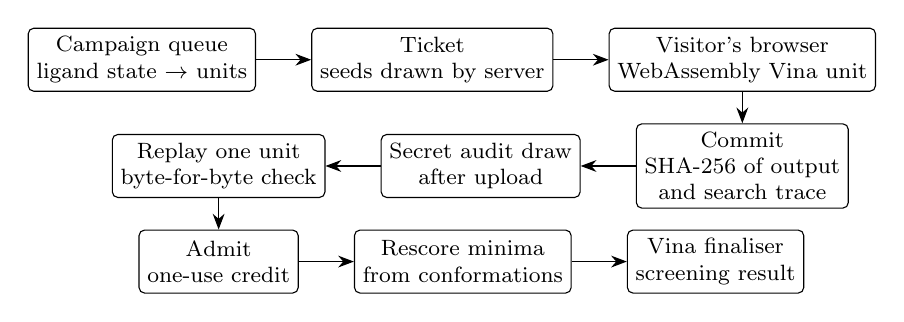
\begin{tikzpicture}[font=\footnotesize,node distance=4mm and 7mm,
  box/.style={draw,rounded corners=2pt,align=center,minimum height=8mm,inner sep=3pt},
  arr/.style={-{Stealth[length=2mm]}}]
\node[box] (queue) {Campaign queue\\ligand state $\rightarrow$ units};
\node[box,right=of queue] (ticket) {Ticket\\seeds drawn by server};
\node[box,right=of ticket] (browser) {Visitor's browser\\WebAssembly Vina unit};
\node[box,below=of browser] (commit) {Commit\\SHA-256 of output\\and search trace};
\node[box,left=of commit] (draw) {Secret audit draw\\after upload};
\node[box,left=of draw] (replay) {Replay one unit\\byte-for-byte check};
\node[box,below=of replay] (admit) {Admit\\one-use credit};
\node[box,right=of admit] (rescore) {Rescore minima\\from conformations};
\node[box,right=of rescore] (final) {Vina finaliser\\screening result};
\draw[arr] (queue)--(ticket);\draw[arr] (ticket)--(browser);\draw[arr] (browser)--(commit);
\draw[arr] (commit)--(draw);\draw[arr] (draw)--(replay);\draw[arr] (replay)--(admit);
\draw[arr] (admit)--(rescore);\draw[arr] (rescore)--(final);
\end{tikzpicture}
\caption{Admission with useful work. The server assigns units with fresh seeds; the browser runs one or more units and commits to their outputs and search traces before learning which unit will be replayed; a secretly drawn unit is replayed exactly; accepted units are rescored and merged by Vina's own finaliser.}
\label{fig:system}
\end{figure}

\subsection{Verification}

Verification is replay. The server re-executes a sampled unit with the same build, inputs and seed and compares output byte for byte. Three measures make that comparison meaningful.

\begin{itemize}
\item \textbf{Output commitment.} A client commits to the SHA-256 of its full output before the audit draw is derived, and the draw is computed server-side from a secret, so a client cannot learn which unit will be replayed before uploading.
\item \textbf{Trace commitment.} The commitment covers a hash of the per-step search trace, not only the final minima pool. Section 5.3 shows why the pool alone is insufficient.
\item \textbf{Fresh seeds.} Each unit's seed is drawn by the server, and a unit re-issued after expiry or failure receives a new seed, so an earlier answer cannot satisfy that new assignment. This prevents ordinary duplicate-answer caching, not every form of precomputation or algorithmic shortcut.
\end{itemize}

Build equivalence was established before any security experiment: three builds from the same sources and flags agreed coordinate for coordinate with an uninstrumented reference on every retained pose, and divergence from the official prebuilt binary was confined to last-bit C runtime differences amplified by Monte Carlo search.

\subsection{Admission tiers}

Newcomers are admitted in bundles of four units, one of which is replayed, so verifier cost is 25\% of client work at one audit draw. An identity that has had three bundles replayed and accepted may enter a trusted tier in which units are audited at a rate p. Each admission grants one single-use credit.

For availability we evaluate, as isolated prototypes rather than the deployed scheduler, stateless authenticated tickets with reserved capacity for established users, an effort-priority queue for newcomers adopted from Tor's onion-service defence~\citep{TorProp327}, and an attested lane for newcomers holding tokens from a mock issuer inspired by Privacy Pass~\citep{Davidson18,RFC9576}. The mock assumes an origin-bound, single-use token with a per-device quota; it does not implement blind signatures or integrate a deployed issuer.

\subsection{Threat model}

Identities are free. The attacker knows the protocol, submits arbitrary bytes, keeps anything it has computed, coordinates across identities and may hold native CPU cores. It cannot forge server commitments or read server secrets. Trust grants and replay verdicts come from trusted server components. We evaluate eight attacker behaviours, fixed in the protocol before any was implemented: zero work (A1), partial work (A2), cached replay (A3), retry grinding (A4), identity reset (A5), disappearing workers (A6), collusion (A7) and subtle scientific corruption (A8). A8 distinguishes useful work from puzzles, because a plausible but wrong result cannot be rejected by a cheap structural check. Attacks on the verifier's host, side channels and compromise of the attestation issuer are out of scope.

\subsection{Security model}

We state the admission guarantee we rely on, and its assumption, rather than prove a general lower bound. A unit u is fixed by its prepared inputs, a server-drawn seed s and an evaluation budget B of 256,000 energy evaluations. Honest execution produces a minima pool P and a trace T = ((e\_1, c\_1), \ldots{}, (e\_n, c\_n)), where e\_i is the energy of the refined candidate at Monte Carlo step i, recorded at full double precision, and c\_i is the cumulative number of energy evaluations. A bundle of four units is accepted if one unit, drawn uniformly by a keyed hash of the ticket and the client's commitment to every unit's pool and trace hash, replays to byte-identical P and T.

\textbf{Assumption (trace work).} For a fresh seed, producing (P, T) equal to the honest output without performing essentially the honest sequence of evaluations succeeds with negligible probability. The committed values are the outcomes of a sequential search in which each step starts from the previous accepted state, and equality is byte-exact, so an approximate or reordered computation changes the committed bytes. We support the assumption empirically (Section 5.3) and discuss its limits in Section 6; we do not prove it.

\textbf{Proposition.} Under the assumption, with a secret draw derived only after commitment and a fresh seed for every re-issued unit, any strategy that computes m of a bundle's four units and fabricates the rest has expected work per admission of four units, the same as honest work, for every m from 1 to 4. \emph{Argument.} The bundle is accepted only if the draw selects a computed unit, which happens with probability m/4 on each attempt. Because the draw is secret and every retry carries fresh seeds, attempts are independent and earlier answers cannot be reused, so the expected number of attempts is 4/m, each costing m units. The flaws measured in Section 5.3 each break one premise: unchanged seeds on retry let computed units be reused, and revealing the draw before upload let a client abandon exactly when selected. The same premises justify treating attempts as independent in the discount-factor intervals. The proposition bounds expected work, not its variance, and says nothing about the scientific quality of the unaudited units, which Section 5.4 examines.

\subsection{Verification time and leverage}

Three quantities characterise a useful-work gate. The verification time V is the verifier's CPU time per admission, including audits; with W verifier cores the gate can check at most W / V admissions per second, the capacity R of Section 5.5. The leverage L is the time the server would need to compute the same useful output itself, with its best native implementation, divided by V: useful work obtained per unit of verifier work. The delivery D is the bytes a client downloads and uploads per admission. Proof of work has V of about a microsecond and no useful output. A docking bundle has V = 1.52 s for four units of work, L = 4, and L = 1/p in the trusted tier, where only a fraction p of units is replayed. These are honest-submission leverages, as are all leverages we report: they assume every admitted unit is useful. Under attack, rejected submissions cost verification and yield nothing, and admitted bundles may carry fabricated units. By the Proposition, an attacker computing m of four units is admitted with probability m/4 per replay and contributes m useful units, so useful work per newcomer replay falls from 4 to m$^2$/4, 0.25 at m = 1; in the trusted tier a fabricating identity yields no useful work for about 1/p units before an audit quarantines it. The classifiers of Section 5.6 check every layer, so fabricated results are rejected rather than admitted, but each rejection still costs V. For docking these values are set by construction: a replay costs the server as much as the unit it checks, so leverage is the inverse of the fraction of work replayed, and what docking measures is the availability cost of that verification (Section 5.5). For a workload checked without replay, leverage is an empirical ratio of two measured times; we always take it against the server's fastest measured option for the same output. Section 5.6 measures V, L and D for a second workload class whose results are checked algebraically rather than by replay.

\section{Methodology}

\subsection{Predeclared protocol}

The evaluation follows a written protocol dated 22 September 2026 and committed to version control on 23 September, before any attack was run. Thresholds could not be revised after outcomes were seen; every change is a dated amendment committed to version control before the experiment it governs, with the original preserved. Eighteen amendments (numbered 1 to 15, with 9b, 14b and 15b) cover phase operationalisation, the three economic fixes, scientific integrity, trace commitment, the rescoring driver, newcomer pricing, attestation, the subpuzzle baseline, a correction of the simulator's replay timing with five-seed replication, a proof-of-work gate baseline, and the verification-leverage study with its phone, batching and native-verifier predictions. Every run manifest records the protocol version it ran under, and a committed audit script confirms that each of the 20 predeclared result sets was produced after the commit of its governing amendment.

The timeline is short, and every step is dated in the public commit history. The docking pipeline was built from 7 September 2026, and the stock qualification and matched campaigns ran from 14 to 23 September; the adversarial protocol was written on 22 September, while the matched campaign was finishing. The later experiments are fast relative to docking: attacks replay units from a fixed corpus, and each availability simulation takes seconds to minutes. Implementation was assisted by coding tools (Section 4.4). Where a prediction failed we report the failure, its cause and any post-hoc diagnostic separately from the predeclared result. The protocol is internally predeclared and timestamped in version control, not lodged with a third-party registry. Amendments chose later experiments in light of earlier results; what they fix in advance is each experiment's predictions and thresholds, not the sequence of experiments. The compressed timeline does not weaken that: each amendment was committed before its experiment ran, which the audit script checks against the run manifests, and every prediction is reported whether it held or failed. What it cannot rule out is that more time would have led to different experiments.

\subsection{Corpus, manifests and statistics}

Attacks run on real molecular output, not synthetic records. The corpus is the set of campaign jobs whose salted hash falls below 5\% of the hash space, a rule fixed before any attack was designed; 33 jobs across all five targets were recovered, containing 4,397 units with raw minima pools, traces and metrics. Every run writes a frozen execution manifest recording protocol, corpus, build and runner hashes, and re-running with a changed input fails. Proportions are reported with exact (Clopper--Pearson) 95\% intervals. Attacker discount factors are ratios of attempt counts; we report 95\% intervals from the geometric distribution of attempts per admission, treating attempts as independent, as Section 3.5 justifies for the fixed scheduler.

\subsection{Measurement boundaries and reproducible methods}

\begin{table}[htbp]
\caption{Evidence supporting the claims and what each experiment does not establish.}
\centering
\small
\begin{tabularx}{\textwidth}{XXX}
\toprule
Claim & Evidence & Boundary \\
\midrule
Screening preservation & Actual native paired docking and finalisation, five panels & Qualified 96-compound panels, not full libraries or prospective biological validation \\
Trace-bound replay & Actual unit re-execution and byte/hash comparison & Tested builds, inputs and attacks; not a computational lower bound \\
Admission economics & Committed scheduler with simulated time and replay-derived verdicts & Specified strategies and cost model; not production traffic \\
Scientific poisoning & Actual corpus re-finalisation; separately, score-shift resampling & Whole-panel AUC effects are exploratory projections \\
Browser feasibility & Real phone execution and reference hash checks & Cooperative sessions, selected repeated units; not client attestation \\
Overload and trust bootstrap & Real queue SQL with modeled arrivals, replay and puzzle costs & Conditional finite-horizon simulations; not measured HTTP throughput \\
Attestation benefit & Mock issuer, token checks and one-use nullifiers & Assumed quota and token supply; no deployed issuer or blind-signature integration \\
Inference leverage & Actual exact-integer verification and native inference timings on one host & Five small models on one laptop-class host; batches to 128 inputs, a laptop GPU and a native dense verifier; no server-class accelerators \\
\botrule
\end{tabularx}
\end{table}

Supplementary Section S1 gives the complete protocols: target selection and input preparation, compute matching and the paired bootstrap, the poisoning projection, and the availability simulator. The availability results use exact replay-event timing and five seeds, correcting an earlier simulator discretisation; the original single-seed results are preserved and compared in Supplementary Section S3.

\subsection{Use of AI tools}

Large language model coding assistants (Anthropic Claude and OpenAI Codex) were used to implement experiment code, analysis scripts and prototypes, to search and verify literature, and to draft text, under the authors' direction. All predictions were committed to version control before the experiments they govern ran; every number in this paper is produced by committed scripts from recorded data; and the authors reviewed the code, results and text and take responsibility for them. The assistants are not authors.

\section{Results}

\subsection{Can docking be decomposed without changing the science?}

Five targets from the DUD-E benchmark~\citep{Mysinger12}, selected from published Vina results before any local run and each a panel of 32 actives and 64 decoys, passed predeclared ranking and redocking gates with stock Vina (ROC-AUC 0.87--0.99). In a matched comparison of 2,073 paired state jobs over three seeds with no failures, every ligand state was docked both as one exhaustiveness-32 run and as independent units merged by the original finaliser, at matched evaluation budget.

\begin{table}[htbp]
\caption{Matched comparison of decomposed and monolithic docking: change in screening ROC-AUC, three seeds, 96-compound panels.}
\centering
\small
\begin{tabularx}{\textwidth}{XrXr}
\toprule
Target & Mean $\Delta$AUC & Paired 95\% interval & Evaluation ratio \\
\midrule
WEE1 & $-$0.0003 & [$-$0.0015, +0.0000] & 1.0040 \\
PUR2 & +0.0033 & [$-$0.0067, +0.0164] & 1.0025 \\
FA7 & +0.0020 & [$-$0.0093, +0.0163] & 1.0034 \\
TGFR1 & $-$0.0008 & [$-$0.0060, +0.0036] & 1.0045 \\
KIF11 & +0.0003 & [$-$0.0042, +0.0049] & 1.0045 \\
\botrule
\end{tabularx}
\end{table}

Every interval lies within $\pm$0.017 and straddles or touches zero; EF10 was identical on 14 of 15 target--seed pairs. Decomposition costs under 0.5\% extra evaluations and no extra search time. The predeclared non-inferiority margin of $-$0.05 is generous relative to these effects, so we read the result from the intervals, not the margin. These are 96-compound panels, not full-library screens.

\subsection{Can browsers reproduce the units, and at what latency?}

In a first study on four phones, all 68 executions of four distinct reference units were bitwise identical to the native reference output across iOS and Android. Against a single hashcash puzzle calibrated on each device to its median unit, 21.9\% of puzzle solves exceeded twice the median and none of 64 warm units did (Supplementary Section S2). Natively, a docking unit also had half the coefficient of variation of a median-matched hashcash puzzle (0.48 against 0.95).

A single hash puzzle is not the strongest baseline: deployed proof-of-work CAPTCHAs split the work into many small puzzles~\citep{FriendlyCaptcha}, and the sum of 64 geometric solve counts is far narrower than one. We therefore ran a second page on five phones, interleaving each unit with two single puzzles and two 64-subpuzzle puzzles, all calibrated on the device to its median unit (amendment 11).

\begin{table}[htbp]
\caption{Five phones, 16 warm units and 24 solves of each puzzle type per phone, pooled by each device's median unit time as predeclared.}
\centering
\small
\begin{tabularx}{\textwidth}{Xrrr}
\toprule
Kind & n & p95/median & Over 2$\times$ median \\
\midrule
Docking unit & 80 & 1.15 & 0\% \\
Single puzzle & 120 & 4.40 & 25.8\% \\
64-subpuzzle puzzle & 120 & 2.02 & 5.8\% \\
\botrule
\end{tabularx}
\end{table}

Two of four predictions held: single puzzles again had a long tail, and units stayed within 1.35 times their median at the 95th percentile. The prediction that subpuzzles would too failed, and so did the calibration check that explains it: on-device calibration missed by up to a factor of 1.66 (Moto Edge 50) and 0.70 (Galaxy M30s), so pooling by unit time mixes shifted distributions. Measured within each device instead, a post-hoc analysis, subpuzzle solves had p95/median 1.14--1.40 and none exceeded twice their own median; pooled, 1.21 against 1.15 for units (Figure 2). As stated before the experiment, lower latency variance is therefore not an advantage of useful work over a well-designed puzzle. It is an advantage only over a single puzzle.

\begin{figure}[htbp]
\centering
\includegraphics[width=0.6\textwidth]{figures/device_latency.pdf}
\caption{Solve time on five phones for docking units, single puzzles and 64-subpuzzle puzzles run in the same sessions. Each time is divided by its device's median for that kind, so the curves compare distribution shape; the dotted line marks twice the median. Calibration error, which this scaling removes, is reported in the text.}
\label{fig:latency}
\end{figure}

The budget phone is 3.7 times slower than the iPhone at docking but 5.2 times slower at JavaScript hashing, and its first contribution takes about 13 s including asset delivery, a real accessibility cost.

All 85 executions in this second study also matched the reference output exactly. These repeat four distinct reference units across the five phones; they are not 85 distinct molecular workloads.

\subsection{Can clients fake the work cheaply?}

\textbf{Unit-level attacks under real replay.} We ran 693 trials on 99 units sampled by salted hash from the corpus, across all five targets.

\begin{table}[htbp]
\caption{Unit-level attacks judged by exact replay, 99 corpus units.}
\centering
\small
\begin{tabularx}{\textwidth}{XrX}
\toprule
Attack & Accepted & 95\% interval \\
\midrule
Honest unit & 99/99 & [0.96, 1.00] \\
A1 substitution of another unit's result & 0/99 & [0.00, 0.04] \\
A3 cached resubmission & 99/99 & by design; one-use credits refuse it \\
A2 quarter work, pool-only commitment & 20/99 & [0.13, 0.30] \\
A2 half work, pool-only commitment & 45/99 & [0.35, 0.56] \\
A2 quarter or half work, pool and trace commitment & 0/198 & [0.00, 0.02] \\
\botrule
\end{tabularx}
\end{table}

Committing to the minima pool alone does not enforce work: the retained minima of a Vina search often stabilise before its budget is spent, so a search stopped at a quarter or half of its evaluations can reproduce the full pool byte for byte. Binding the per-step trace rejected every tested quarter- and half-budget submission. This tests those truncation strategies, not a general computational lower bound. Hashing the trace preserves the tested replay check, subject to collision resistance, while cutting median upload from 163 KB to 19 KB. Falsifying the best energy by 0.1--3.0 kcal/mol never changed any output, because the finaliser recomputes energies; moving the best pose by 0.1 or 0.5 \AA{} had no effect.

\textbf{Admission economics with free identities.} We define the attacker discount factor as attacker work per admission divided by honest work per admission in the same tier. A hash puzzle is normalised to 1.0 under a common hardware and expected-hash cost model; that is not a claim of equal wall time or energy across hardware. Below 1.0, the modeled attacker cost is lower than the honest cost. On the committed scheduler, 118 configurations were run with audit verdicts resampled from real replay records.

As first built, the scheduler had three flaws. Abandoned units returned with the same seed, so an attacker who computed one of four units reused it until the audit draw landed on it. The audit draw was revealed before upload, so a trusted identity could abandon exactly when selected and never be caught. And trust was granted after one bundle. Each fix was predeclared and measured separately.

\begin{table}[htbp]
\caption{Attacker discount factor on the committed scheduler before and after the three fixes.}
\centering
\small
\begin{tabularx}{\textwidth}{XrXX}
\toprule
Configuration & Before & After, 95\% interval & Predicted \\
\midrule
Bundle tier, attacker computes 1 of 4 units & 0.46 & 0.96 $\pm$ 0.09 & 0.95--1.10 \\
Bundle tier, attacker computes 2 of 4 units & 0.57 & 1.03 $\pm$ 0.08 & 0.95--1.10 \\
Bundle tier, attacker computes 3 of 4 units & 0.76 & 1.00 $\pm$ 0.06 & 0.95--1.10 \\
Trusted tier, trust after 1 bundle, p = 0.02--0.25 & 0.44--1.19 & 0.44--1.40, reveal removed & analytic, matched \\
Trusted tier, trust after 3 audited bundles & --- & 1.36--4.04 & at least 1.0 \\
\botrule
\end{tabularx}
\end{table}

With reseeding, no reveal and a three-bundle threshold, the large observed bundle-tier discounts disappear, and the estimates are consistent with parity under the evaluated cost model. The lowest interval, 0.96 $\pm$ 0.09, also permits a modest attacker advantage; containing 1.0 does not establish equality or a lower bound of 1.0. Identities are free in these experiments, but results apply to the specified strategies, attempt model and workload costs, not every possible adversary. Before the fixes, compensating for the measured discounts would have required an identity price of 0.5--5.1 honest units. The fixes remove the particular reuse, disclosure and early-trust paths responsible for those discounts.

Capacity exhaustion by workers who accept units and disappear behaved as a threshold rather than proportionally: holders of 4, 8 and 12 of 16 leases caused no refusals, and 16 caused 81\%. Stateless tickets that allocate seeds without reserving queue seats removed the effect in the isolated prototype.

Every behaviour in the threat model is covered, though not all by a dedicated experiment: A1--A3 above, A4 and A5 by the free-identity admission strategies, A6 by lease exhaustion and A8 in Section 5.4. Collusion (A7) was not run separately; a result computed for another unit fails replay like substitution, and resubmission is refused by one-use credits. Supplementary Section S4 lists the further scheduler configurations: attempt caps, two audit draws, reduced-budget units and trust acquisition.

Section 6 discusses what trace commitment does and does not establish about the work an accepted unit requires.

\subsection{Can fabricated work corrupt the science?}

We ran the original finaliser over saved corpus pools with units replaced or altered. This offline experiment measures damage conditional on malicious outputs entering the aggregate; it does not demonstrate a way to bypass the admission scheduler. In the scheduler, a bundle rejected by immediate audit does not enter the scientific pool. Unaudited outputs in accepted bundles and outputs admitted before deferred audit are distinct exposure paths.

\begin{table}[htbp]
\caption{Corpus re-finalisation measurements; the ROC-AUC entry is a separate exploratory projection.}
\centering
\small
\begin{tabularx}{\textwidth}{XX}
\toprule
Experiment & Measured \\
\midrule
Units with the wrong atom count & rejected 33/33 \\
Stored coordinates moved 2 \AA{}, conformation untouched & $-$0.10 to +0.02 kcal/mol, within the predicted 0.12 \\
Conformation moved 2 \AA{}, coordinates untouched & $-$0.42 to +1.37 kcal/mol; the prediction of no gain failed \\
Honest duplication of 5--75\% of units & measured best gain $-$0.10 kcal/mol; projected mean ROC-AUC change within $\pm$0.002, and every 95\% envelope within $\pm$0.009, up to 75\% \\
Duplicated units claiming $-$20 kcal/mol, 5\% of units & 22 of 33 jobs worse (95\% interval 0.48--0.82), by up to 1.859 kcal/mol \\
\botrule
\end{tabularx}
\end{table}

In these tests, fabricated reported energies did not survive final rescoring: the finaliser recomputed the output energies from conformations. This does not establish biological validity or rule out false positives in screening. The largest score improvement across these pool-tampering experiments was 0.466 kcal/mol, in the 5\% fabricated-energy condition. The largest worsening was 2.632 kcal/mol at 10\% corruption, compared with 1.859 at 5\%. The merge still ranks and clusters minima by the energies clients report and keeps a bounded set for refinement, so fabricated minima displace honest ones before refinement sees them. In an exploratory, non-predeclared resampling projection, mean ROC-AUC changes reached about $-$0.016 at 5\% and $-$0.034 at 10\% fabricated units. These are not measured whole-panel poisoning outcomes: corpus score shifts were resampled onto otherwise unchanged campaign scores (Supplementary Section S1). A revised driver that rescores every submitted minimum from its conformation before merging was verified against the same gates.

\begin{table}[htbp]
\caption{Rescoring driver against the original driver.}
\centering
\small
\begin{tabularx}{\textwidth}{XXX}
\toprule
Check & Original & Rescoring \\
\midrule
Build-equivalence gates and replay, five targets & pass & pass \\
Honest pools finalised & --- & byte-identical, 33/33 \\
Falsified-energy attack, projected mean $\Delta$AUC & as low as $-$0.034 & within $\pm$0.0016 \\
Jobs worsened at 5\% falsified units & 22/33 & 2/33, as honest duplication \\
Jobs changed by coordinate-only tampering & 16/33 & 0/33 \\
Rescoring overhead per ligand state & --- & +91 ms median; 0.046\% relative to calibrated client work \\
\botrule
\end{tabularx}
\end{table}

The $\pm$0.0016 AUC range is also a projection. Rescoring addresses fabricated energy ordering; it does not certify that unaudited pools contain all minima that honest search would have found. \textbf{Contamination at scale.} Rescoring removes fabricated energies but not missing search. In the newcomer tier, where every bundle is audited before admission, an attacker who computes m of a bundle's four units is admitted only when the audit lands on a computed unit (Section 3.5), so each admitted attacker bundle carries 4 $-$ m fabricated units, at most three, into the pool. If attackers hold a share s of admitted bundles, the fraction of admitted units that are fabricated is s(4 $-$ m)/4 and the useful yield per admission is 1 $-$ s(4 $-$ m)/4. At s = 1 and m = 1, 75\% of admitted units are fabricated and the useful yield is 25\%; no newcomer bundle can carry more, since m = 0 is never admitted. The trusted tier, which admits bundles on history without auditing each one, has no such bound until a failed audit quarantines the identity. The duplication experiment covers the newcomer range for missing search spread across a job's units: replacing up to 75\% of them with duplicates, which add no new minima, moved projected mean ROC-AUC by at most 0.002 on every target, with 95\% envelopes within $\pm$0.009. Under those conditions, with energies rescored, contamination slowed the campaign, requiring up to four times as many admissions per ligand, without measurably changing its rankings. It does not cover attacks that concentrate missing search on particular compounds, such as suppressing likely actives, which could change rankings and were not tested.

\subsection{What does useful work cost compared with proof of work?}

A hashcash puzzle calibrated natively to a similar median client time (1.38 s against 1.52 s for a unit) verifies in 0.77 $\mu$s. Verifying useful work costs a replay of 1.52 s for each audited unit, a fraction q of client work: about five orders of magnitude more at q = 0.1. The puzzle also guarantees freshness, which useful work must restore with assignment seeds and one-use credits. The rest of this section asks what that verification cost does under attack.

Each fake submission selected for audit costs the verifier a 1.52 s replay. Let R be the verifier's replay capacity in replays per second, $\lambda$ the honest newcomer arrival rate, r a device's hash rate and T the time a visitor will spend bidding. An honest bid is about rT hashes, so an attacker who buys the spare R $-$ $\lambda$ replay slots each second at that price needs a hash budget of about (R $-$ $\lambda$) $\cdot$ r $\cdot$ T. We use this as a capacity model, not a sharp cutoff, and tested it on an effort-priority queue following Tor's design, driving the real queue code with measured phone and native rates, 40 honest newcomers per device class and five seeds (Figure 3). The model's predictions held in 230 of 240 checks; every check, and how these results relate to an earlier single-seed run, is in Supplementary Section S3.

At eight replay workers the queue discriminates sharply by device. Against a four-core attacker, mean service was 0.070, 0.965 and 1.000 for budget, mid-range and flagship phones; against sixteen cores, 0.110, 0.135 and 0.130.

\begin{figure}[htbp]
\centering
\includegraphics[width=\textwidth]{figures/served_vs_cores.pdf}
\caption{Corrected full-patience simulation: mean service across five seeds, with shading for the observed minimum--maximum range. Dashed lines mark the conditional budget scale $(R-\lambda)\,r\,T$, not a guaranteed cutoff. Grey dotted: the same queue with proof-of-work verification, lowest-served device class. Input polling remains discrete; replay completion uses exact event times.}
\label{fig:served}
\end{figure}

\textbf{Proof-of-work gate baseline.} To isolate what replay adds, amendment 13 reran the same queue, arrivals, device and attacker rates, bidding strategies and seeds with verification costing the measured 0.77 $\mu$s hash check instead of a 1.52 s replay (360 runs). Both predictions held. Every device class was at least 90\% served, as a five-seed mean, in all 72 cells up to 16 attacker cores. In the 23 cells where useful-work service fell below 0.2 for some class, the proof-of-work gate served every class at 0.95--1.00; at eight workers and 16 cores the lowest-served class went from 0.110 to 0.950 (Figure 3). The gate itself never became the bottleneck. This baseline models the gate only: under proof of work an attacker who pays the puzzle is admitted and loads the protected service behind it, which we did not simulate. The comparison therefore isolates the availability price of replay verification rather than comparing whole deployments.

A native core hashes about 36 times faster than the budget phone's JavaScript, and pricing alone does not remove that disparity. Because trust requires three audited bundles, newcomers who are outbid cannot earn trust either: under a sixteen-core attack without attestation, no budget or mid-range newcomer reached trust, and flagship newcomers did so at a mean of 0.030.

\textbf{Outside trust.} If an issuer supplies origin-bound, one-use tokens with a per-device quota, a separate replay lane lets token holders earn trust without winning the hash auction. We model the issuer with a mock; this is not a deployed Privacy Pass integration. At an assumed 90\% honest token coverage, every attested group reaches trust in all five seeds at attacker supply 0, 0.1 or 1 tokens/s with eight workers. At zero attacker tokens, mean within-seed median trust times are about 66 / 23 / 23 s, conditional on success and excluding the initial bundle's molecular work, which is already available at first arrival in this harness. Later bundles include device-calibrated work time. At ten attacker tokens per second, trust fractions fall and vary across seeds and device classes (Supplementary Table S4).

\begin{figure}[htbp]
\centering
\includegraphics[width=\textwidth]{figures/trust_bootstrap.pdf}
\caption{Corrected mock-attestation simulation under sixteen attacker cores. Bars show five-seed mean trust fractions; whiskers show observed minimum--maximum ranges. Left of the grey line: no attestation. Right: 90\% honest token coverage as assumed attacker token supply rises. The issuer and token-acquisition budgets are modeled.}
\label{fig:trust}
\end{figure}

Cheap attacker tokens consume attested replay capacity ahead of anonymous visitors, and the benefit rests on the assumed issuer quota and token supply.

\subsection{Does cheaper verification escape the trade-off?}

Replay makes docking's verification expensive. To test whether that is a property of useful work or of replay, we added a workload verified algebraically: image classification for data labelling. A client runs a small classifier in exact integer arithmetic and uploads every affine layer's output; the verifier checks each layer with four secret Freivalds projections~\citep{Freivalds77}, as in Slalom~\citep{Tramer19}, and recomputes only the cheap nonlinear operations. We measured five models, from a 110-thousand-parameter MNIST perceptron to VGG11-BN on CIFAR-10.1 and a perceptron with two 2,048-wide layers, against the server's best native inference (Table 8, Supplementary Section S6).

\begin{table}[htbp]
\caption{Verification leverage of five labelling models. C is the server's best native inference time and V the verification time, including parsing, hashing, range checks, projections, nonlinear operations and an 8\% audit rate; leverage L is C/V, shown without audits and at an 8\% audit rate. Accuracy is the quantized model's test accuracy.}
\centering
\small
\begin{tabularx}{\textwidth}{Xrrrrr}
\toprule
Model & Acc. & C / V (ms) & L, 0\% / 8\% & Trace & Weights \\
\midrule
MNIST MLP & 96.8\% & 0.078 / 0.219 & 0.37 / 0.36 & 0.8 KB & 0.11 MB \\
MNIST CNN & 98.7\% & 0.262 / 0.377 & 0.73 / 0.69 & 37.9 KB & 0.05 MB \\
CIFAR CNN & 76.2\% & 0.985 / 1.13 & 0.93 / 0.87 & 115.2 KB & 0.16 MB \\
VGG11-BN & 83.1\% & 3.87 / 5.69 & 1.08 / 0.68 & 610.3 KB & 9.76 MB \\
Wide MNIST MLP & 97.6\% & 1.60 / 1.12 & 1.80 / 1.43 & 16.4 KB & 5.84 MB \\
\botrule
\end{tabularx}
\end{table}

All three predictions about correctness and ordinary models held: every perturbation of every trace was rejected, and the four ordinary models reached leverage 0.36--0.87 at an 8\% audit rate, below the predicted 1.5. For the smallest models the verifier spends more than it would to compute the answer. The prediction that the wide perceptron would reach leverage 10 failed: it reached 1.80 without audits and 1.43 with them. That prediction came from an earlier micro-benchmark that compared checking with an exact double-precision baseline; against optimised native inference, a 2,048-wide layer computes in about a millisecond, and the verifier's fixed per-layer work of parsing, hashing and range checking, not the projections themselves, dominates.

Cheap verification does fix availability. Rerunning the admission grid with each model's verification time in place of the replay kept every device class at least 90\% served in all 360 cells up to sixteen attacker cores, as the proof-of-work gate did. What it does not provide is leverage. Figure 5 places every measured workload by verification time and leverage: proof of work at a microsecond with no useful output, the classifiers at 0.2--6 ms with leverage near one, and docking at honest-submission leverage 4 and 10 with 152--1,520 ms of verification. No workload we measured is both cheap to verify and high in leverage.

Two further amendments asked whether batch size or the verifier's implementation, rather than the method, set that limit. In amendment 15 each admission labelled a batch of up to 128 inputs, verified with the same secret projections as matrix products. Leverage fell with batch size for every model: batching made the server's own inference cheaper per input faster than it made verification cheaper, and in convolutional networks, where most output values come from early layers with only 9 to 576 multiply-accumulates each, the verifier's work per value dominates. A GPU baseline was slower than one CPU thread at small batches, from launch and transfer overhead, so leverage measured against the GPU alone reached 2.7 for the MNIST perceptron's single inputs, 0.31 against the server's fastest option, one CPU thread; against the GPU it fell below 1 for every model at 128 inputs. In amendment 15b a native kernel verified a whole dense network per call, with an exact native audit, and the native forward pass joined the server's baselines. It was exact, but the wide perceptron reached leverage 2.21 at 8\% audits against the server's fastest option, the GPU, and 3.15 had the server no GPU, short of the predicted 4; the 2.2 quoted elsewhere is the former. What remains is per-admission work that does not shrink with the layer: hashing the trace, quantising the input, entering native code with cold caches, and the audits. Of the eight predictions in the two amendments, three held: exactness in both, and the narrow perceptron staying below 4 (Supplementary Section S6).

\begin{figure}[htbp]
\centering
\includegraphics[width=0.75\textwidth]{figures/design_space.pdf}
\caption{Verifier time per admission against verification leverage for every measured workload. All leverage is for honest submissions; docking's is set by its audit rate and falls under attack (Section 3.6). The open circle is the wide perceptron with the native verifier of amendment 15b. The shaded region, cheap to verify with leverage above four, contains no measured workload.}
\label{fig:design}
\end{figure}

We then ran the five classifiers on four of the study phones in exact integer JavaScript, three inputs and three repetitions each, followed by the SHA-256 puzzle rate and eight evaluations of scrypt~\citep{RFC7914}, a memory-hard function using 16 MB (N = 16384, r = 8, p = 1), as a proof-of-work baseline that the earlier studies lacked. Three predictions were recorded before the page ran (amendment 14b), and all held. All 270 classifier traces matched the server's expected hashes bit for bit, so algebraic verification needs no tolerance for device arithmetic. The budget phone's gap to one native core was 8.0$\times$ for scrypt against 34.7$\times$ for SHA-256, less than a third, as predicted (Table 9), though the two native references were measured under different load (Supplementary Section S6). The budget phone took 5.7$\times$ as long as the iPhone 15 for VGG11-BN.

\begin{table}[htbp]
\caption{Phone timings for the proof-of-work baselines and the largest classifier; medians over each phone's runs. Gap is native speed on one server core divided by phone speed: 1.25 million SHA-256 hashes per second and 62.4 ms per scrypt.}
\centering
\small
\begin{tabularx}{\textwidth}{Xrrrrr}
\toprule
Phone & SHA-256/s & Gap & scrypt (ms) & Gap & VGG11-BN (ms) \\
\midrule
iPhone 15 & 368066 & 3.4 & 96 & 1.5 & 255 \\
Galaxy A57 & 153501 & 8.1 & 168 & 2.7 & 443 \\
Infinix Note 40 Pro & 69678 & 17.9 & 371 & 6.0 & 718 \\
Galaxy M30s (2019) & 36063 & 34.7 & 500 & 8.0 & 1458 \\
\botrule
\end{tabularx}
\end{table}

A memory-hard puzzle therefore cuts an attacker core's advantage over the budget phone about fourfold; since the capacity model of Section 5.5 scales a device's protection with its rate relative to an attacker core, the budget phone gains the same factor at a puzzle gate. It does not remove device disparity: the spread from budget phone to flagship fell from 10.2$\times$ under SHA-256 to 5.2$\times$ under scrypt, similar to the 5.7$\times$ spread for labelling work on the same phones.

\section{Discussion}

\textbf{The trade-off.} The two workloads fall at opposite ends of one trade-off (Figure 5): docking buys leverage by paying for replay, and the classifiers are cheap to check because they are cheap to compute. A useful workload in the empty region of Figure 5 would need results that are expensive to produce and cheap to check with a certificate, as a hash preimage is for proof of work. Search problems with succinct certificates have that shape; docking's search does not, because its best pose carries no proof that the search was done. Neither batching nor an optimised verifier moved a classifier into that region, but both were measured on laptop-class hardware; wider dense layers or server-class accelerators, which change both sides of the ratio, may land elsewhere in Figure 5.

\textbf{When is useful work worth it?} Only when someone needs the output and the verifier can afford replay. A puzzle is strictly better on verifier cost and freshness; useful work is no more predictable than a subpuzzle puzzle, closes attacker discounts only after the tested fixes, and pays a replay for every fake submission. What it buys is that the visitor's computation docks real ligands instead of being discarded.

\textbf{What trace commitment does and does not establish.} The committed trace records, for every Monte Carlo step, the refined candidate's energy at full double precision and the cumulative number of energy evaluations. A matching trace binds these recorded per-step values, which replay compares byte for byte. It does not record every intermediate energy evaluation, coordinate or gradient, and therefore does not uniquely establish the internal sequence of computations. Two routes to a cheaper accepted trace remain open. Faster hardware or a faster implementation of the same operations, such as native code, vectorisation or a GPU, is not a shortcut in the security sense: it is the same hardware disparity proof of work already has, and Section 5.5 prices it. Avoiding evaluations is the real question. Each committed energy is the end of a local optimisation that starts from a random perturbation of the previous accepted state, and whether that step is accepted decides where the next one starts, so every recorded value depends on the full path of evaluations before it. Matching the trace without the evaluations means predicting a chaotic floating-point trajectory for a fresh seed, not only its end point. Approximate energies, reordered arithmetic or incremental updates change rounding and hence the committed bytes, and fresh server-drawn seeds make one unit's intermediate states unlikely to recur in another. Reusing the precomputed grid maps across units is not a shortcut, since honest clients reuse them too. We tested truncation only; approximate scoring and cross-unit reuse attacks remain untested. We know of no method that yields a matching trace with fewer evaluations than the honest search, but we have not proved that none exists. A lower bound of that kind, for example showing that any accepted trace of N steps requires $\Omega$(N) evaluations under stated assumptions about the scoring function, remains open. Hashcash also rests on an assumption rather than a proof, that SHA-256 admits no shortcut to a preimage below the target, but one backed by decades of public cryptanalysis; the trace-work assumption is backed only by the attacks tested here, so we state it as an assumption and an open question, not an equivalent guarantee.

\textbf{What the useful output is worth.} Docking's honest-submission leverage is four units per replay in the newcomer tier and 1/p in the trusted tier, and less under attack (Section 3.6). A ligand state needs a median of 140 units, about 35 newcomer admissions or 140 trusted admissions, and 140 units are roughly 213 native core-seconds. At an assumed cloud price of 0.04 US dollars per core-hour, one newcomer admission donates about six core-seconds, under a hundredth of a US cent of compute, similar to what a puzzle wastes. The case for useful admission is therefore not revenue. It is that computation a gate would spend anyway produces science instead of heat, at the cost of the verifier capacity Section 5.5 prices.

\textbf{Attacker scale.} Sixteen cores is a small attacker, about 0.64 US dollars per hour at the same assumed price. The capacity model scales directly: to keep a device class served, spare replay capacity must grow by 1.25 million / (r $\cdot$ T) replays per second for every attacker core, 1.25 million hashes per second being the measured native rate of one core. Each replay occupies a verifier core for 1.52 s, so the replay cores needed per attacker core are 1.52 $\times$ 1.25 million / (r $\cdot$ T). With measured rates this is about 5.4 replay cores per attacker core for the budget phone, 1.3 for the mid-range phone and 1.0 for the flagship. Defending budget phones against a botnet therefore requires replay capacity several times the attacker's CPU. This is the price of utility stated as a ratio, and it is the regime in which an outside trust signal, rather than more replay, has to carry the defence. Memory-hard puzzles narrow this gap at its source (Section 5.6).

\textbf{Identity cost.} Proof of work is indifferent to identities; our first scheduler's security depended on identities costing 0.5--5.1 honest units (Section 5.3). We regard this as the most transferable lesson for any useful-work admission design: every retry, reveal and trust path must be checked with identities priced at zero.

\textbf{Reputation under load.} Verifying reputed submitters first protects them: in the isolated ticket prototype, a flood of fake submissions paying a 16-bit puzzle cut newcomers to 1 of 60 served while established users, holding reserved replay capacity, stayed at 60 of 60 (arrivals and replay simulated), and a failed audit quarantines a reputed submitter who turns malicious. It cannot rescue honest newcomers, who have no more history than attackers; that is the trust-bootstrap lockout of Section 5.5, and separating them needs an outside signal such as attestation or the cross-site behavioural signals of deployed challenge services~\citep{Turnstile22}, which trade privacy for discrimination. Against sleeper identities aged during quiet periods~\citep{Douceur02}, useful admission changes the price: earning trust requires three replayed bundles, so pre-built reputation is paid for in real, audited docking. We have not measured a sleeper-identity attack.

\textbf{Consent.} Given the history of covert browser mining (Section 2.2), a useful-work gate that spends visitors' energy must say so, and it gives them a reason a puzzle cannot.

\textbf{Limitations.} Five phone models (four for the classifier and scrypt timings), two workload classes, five 96-compound panels and five small classifiers measured on one laptop-class host. Availability mechanisms are isolated prototypes, not integrated into the deployed scheduler, and their puzzle costs were accounted from measured rates rather than executed. Corrected five-seed results retain substantial anonymous-newcomer denial at sixteen attacker cores, and the mock-attestation lane helps only under assumed honest coverage and attacker token budgets; issuer quotas and platform availability are external requirements. Discount-factor intervals assume independent attempts, which Section 3.5 argues but does not prove. The trusted tier grants unaudited admissions on history, not on the unit. The scheduler quarantines contributors after failed replay and blocks aggregate-output retrieval when their contributions are present. A dedicated late-failure test covers this guard; automatic campaign repair and retraction of already-produced scientific results have not been demonstrated. The rescoring driver is a verified candidate, not yet serving traffic. Pool poisoning AUCs are projections based on exchangeable corpus score shifts, and contamination targeted at particular compounds was not tested. The availability replication measures five-seed variability but keeps arrival rates, device speeds, replay cost and attacker strategies fixed. Puzzle RNGs are seeded; prototype ticket identifiers and their tie-breaking remain cryptographically random. The initial bootstrap bundle is assumed ready at arrival. There is no integrated production traffic or energy-cost validation.

\section{Conclusion}

Useful computation can stand in for discarded proof of work at a browser gate, but verification changes the economics of admission. In the two workload classes we measured, the work worth delegating was expensive to verify and the work cheap to verify was not worth delegating; a workload whose results carry a cheaply checkable certificate is the natural test of whether that holds more generally. Bounded Vina units preserve screening performance and reproduce exactly on phones, and the tested fixes leave attacker cost near parity, not provably so. Replay verification still consumes capacity that a proof-of-work gate does not, overload falls first on budget devices, and external attestation helps only under issuer and token-supply assumptions. These results quantify the practical costs and limits of useful-work admission rather than establish a universal replacement for proof of work.

\backmatter
\section*{Abbreviations}

AUC: area under the curve; BFGS: Broyden-Fletcher-Goldfarb-Shanno; CAPTCHA: Completely Automated Public Turing test to tell Computers and Humans Apart; CDN: content delivery network; CIFAR: Canadian Institute for Advanced Research image dataset; CNN: convolutional neural network; CPU: central processing unit; DUD-E: Directory of Useful Decoys, Enhanced; GPU: graphics processing unit; HTTP: Hypertext Transfer Protocol; MLP: multilayer perceptron; MNIST: Modified National Institute of Standards and Technology handwritten-digit dataset; PoW: proof of work; RNG: random number generator; ROC: receiver operating characteristic; SHA-256: Secure Hash Algorithm, 256-bit; SQL: Structured Query Language; VGG: Visual Geometry Group network.

\section*{Declarations}

\paragraph{Supplementary information}

Additional file 1 (PDF): Supplementary Information. Complete experimental methods (S1), the first four-phone timing study (S2), and all availability prediction checks, five-seed service and trust tables and historical comparisons (S3), further admission-economics configurations (S4), the proof-of-work gate baseline (S5), and the inference-leverage methods (S6).

\paragraph{Availability of data and materials}

An anonymised copy of the repository, including protocol amendments, runners, manifests, analysis scripts, the result ledgers and the figure and manuscript builders, is available for review at \url{https://anonymous.4open.science/r/uwa-review-C3D9/}. The public repository and the archived Zenodo record are withheld to preserve anonymity and will be cited in the final version.

\paragraph{Ethics approval and consent to participate}

Not applicable. All phone timing tests were run by the authors on phones they own. The test page submitted the device model and operating system as entered, the browser user agent and performance measurements; the study stored no names, contact details or location data.

\paragraph{Consent for publication}

Not applicable.

\paragraph{Competing interests}

The authors declare that they have no competing interests.

\paragraph{Funding}

Not applicable.

\paragraph{Authors' contributions}

Withheld for double-anonymous review.

\paragraph{Acknowledgements}

Not applicable.

\bibliography{references}
\end{document}
